%%% Содержимое слайдов

\frame[plain]{\titlepage} % Титульный слайд

%-------------------------------------------------------------------------------

\section{Цели и задачи исследования}

\begin{frame}
\frametitle{\insertsection}

\textbf{Цель:} повышение эффективности процессов обеспечения информационной безопасности облачных сред

\vspace{\baselineskip}

\textbf{Задачи:}
\begin{itemize}
    \item обзор составных частей облачной инфраструктуры
    \item анализ технологий используемых облачными поставщиками
    \item исследование специфики применений облачных вычислений в России
    \item исследование проблем безопасности облачных вычислений
    \item исследование уязвимостей в облачной среде
\end{itemize}
\end{frame}

%-------------------------------------------------------------------------------

\section{Входные и выходные данные}

\begin{frame}
\frametitle{\insertsection}

\textbf{Входные данные:}
\begin{itemize}
    \item структура и характеристики облачной среды
    \item перечень угроз и уязвимостей
    \item перечень характеристик качества системы ИБ
    \item облачная инфраструктура
\end{itemize}

\vspace{\baselineskip}

\textbf{Выходные данные:}
\begin{itemize}
    \item структура системы информационной безопасности
    \item ПО для получения данных об уязвимостях
    \item анализ ПО используемого в облачных вычислениях
    \item информация о проблемах безопасности в облачной среде
\end{itemize}
\end{frame}

%-------------------------------------------------------------------------------

\section{Составные части и технологии облачной инфраструктуры}

\begin{frame}
\frametitle{\insertsection}

\textbf{Составные части:}
\begin{itemize}
    \item клиентские устройства
    \item сетевая среда доступа
    \item специализированное ПО
    \item центр обработки данных
\end{itemize}

\vspace{\baselineskip}

\textbf{Технологии:}
\begin{itemize}
    \item виртуализация
    \item оркестратор
    \item список (каталог) услуг
    \item портал самообслуживания
    \item система тарификации и выставления счетов (биллинг)
\end{itemize}
\end{frame}

%-------------------------------------------------------------------------------

\section{Проблемы стандартизации облачных вычислений}

\begin{frame}
\frametitle{\insertsection}

\textbf{Проблемы:}
\begin{itemize}
    \item не существует единого стандарта безопасности
    \item множество корпоративных стандартов
    \item репутация компании играет важную роль
\end{itemize}

\begin{figure}
    \center
    
\includegraphics[width=\linewidth]{logos}
\end{figure}
\end{frame}

%-------------------------------------------------------------------------------

\section{Стратегически важные области безопасности}

\begin{frame}
\frametitle{\insertsection}
\framesubtitle{Security Guidance for Critical Areas of Focus in Cloud Computing}

\begin{itemize}
    \item архитектурные решения сред облачных вычислений
    \item государственное и корпоративное управление рисками
    \item легальное и электронное открытие
    \item соответствие техническим условиям и отчетность
    \item управление жизненным циклом информации
    \item портативность и совместимость
    \item традиционная безопасность, восстановление
    \item работа центра обработки данных
    \item реакция на риски, уведомление и обучение
    \item прикладная безопасность
    \item криптография и управление ключами
    \item идентификация и управление доступом
    \item виртуализация
\end{itemize}
\end{frame}

%-------------------------------------------------------------------------------

\section{Специфика российского рынка облачных услуг}

\begin{frame}
\frametitle{\insertsection}
\begin{itemize}
    \item наблюдается большой рост
    \item отсутствует явный монополист
    \item рынок облачных услуг разнообразен
    \item качество услуг растет
    \item влияние ФЗ №242-ФЗ <<О внесении изменений в отдельные законодательные акты Российской Федерации в части уточнения порядка обработки персональных данных в информационно-телекоммуникационных сетях>>
\end{itemize}
\end{frame}

%-------------------------------------------------------------------------------

\section{Крупнейшие поставщики услуг ЦОД в России}

\begin{frame}
\frametitle{\insertsection}
\begin{table}[H]
  \begin{tabular}{|p{0.3cm}|p{2cm}|p{2cm}|p{2.3cm}|p{2.6cm}|}
  \hline \# & Название компании & Количество доступных стойко-мест & Количество размещенных стойко-мест & Загруженность мощностей (\%) \\
  \hline 1 & Ростелеком & 3 900 & 3 432 & 88 \\
  \hline 2 & DataLine & 3 703 & 2 988 & 81 \\
  \hline 3 & DataPro & 3 000 & нет данных & нет данных \\
  \hline 4 & Linxtelecom & 2 040 & нет данных & нет данных \\
  \hline 5 & Selectel & 1 500 & 1 200 & 80 \\
  \hline 6 & Stack Group & 1 400 & 854 & 61 \\
  \hline 7 & Ай-Теко & 1 200 & 960 & 80 \\
  \hline
  \end{tabular}
\end{table}
\end{frame}

%-------------------------------------------------------------------------------

\section{Проблемы безопасности в облачной среде}

\begin{frame}
\frametitle{\insertsection}

\begin{itemize}
    \item утечка данных
    \item компрометация учетных записей и обход аутентификации
    \item взлом интерфейсов и API
    \item уязвимость используемых систем
    \item кража учетных записей
    \item инсайдеры-злоумышленники
    \item целевые кибератаки
    \item перманентная потеря данных
    \item недостаточная осведомленность
    \item злоупотребление облачными сервисами
    \item DDoS-атаки
    \item совместные технологии, общие риски
\end{itemize}
\end{frame}

%-------------------------------------------------------------------------------

\section{Результаты системного анализа}

\begin{frame}
\frametitle{\insertsection}

\textbf{Функции:}
\begin{itemize}
    \item авторизация и аутентификация пользователей
    \item сетевая защита
    \item идентификация и обработка инцидентов
    \item предоставление доступа к услугам
    \item мониторинг
\end{itemize}

\vspace{\baselineskip}

\textbf{Подсистемы:}
\begin{itemize}
    \item подсистема аутентификации
    \item подсистема авторизации
    \item подсистема сетевой защиты
    \item подсистема проверки целостности данных
\end{itemize}
\end{frame}

%-------------------------------------------------------------------------------

\section{Принцип иерархий}

\begin{frame}
\frametitle{\insertsection}

\begin{figure}
    \center
    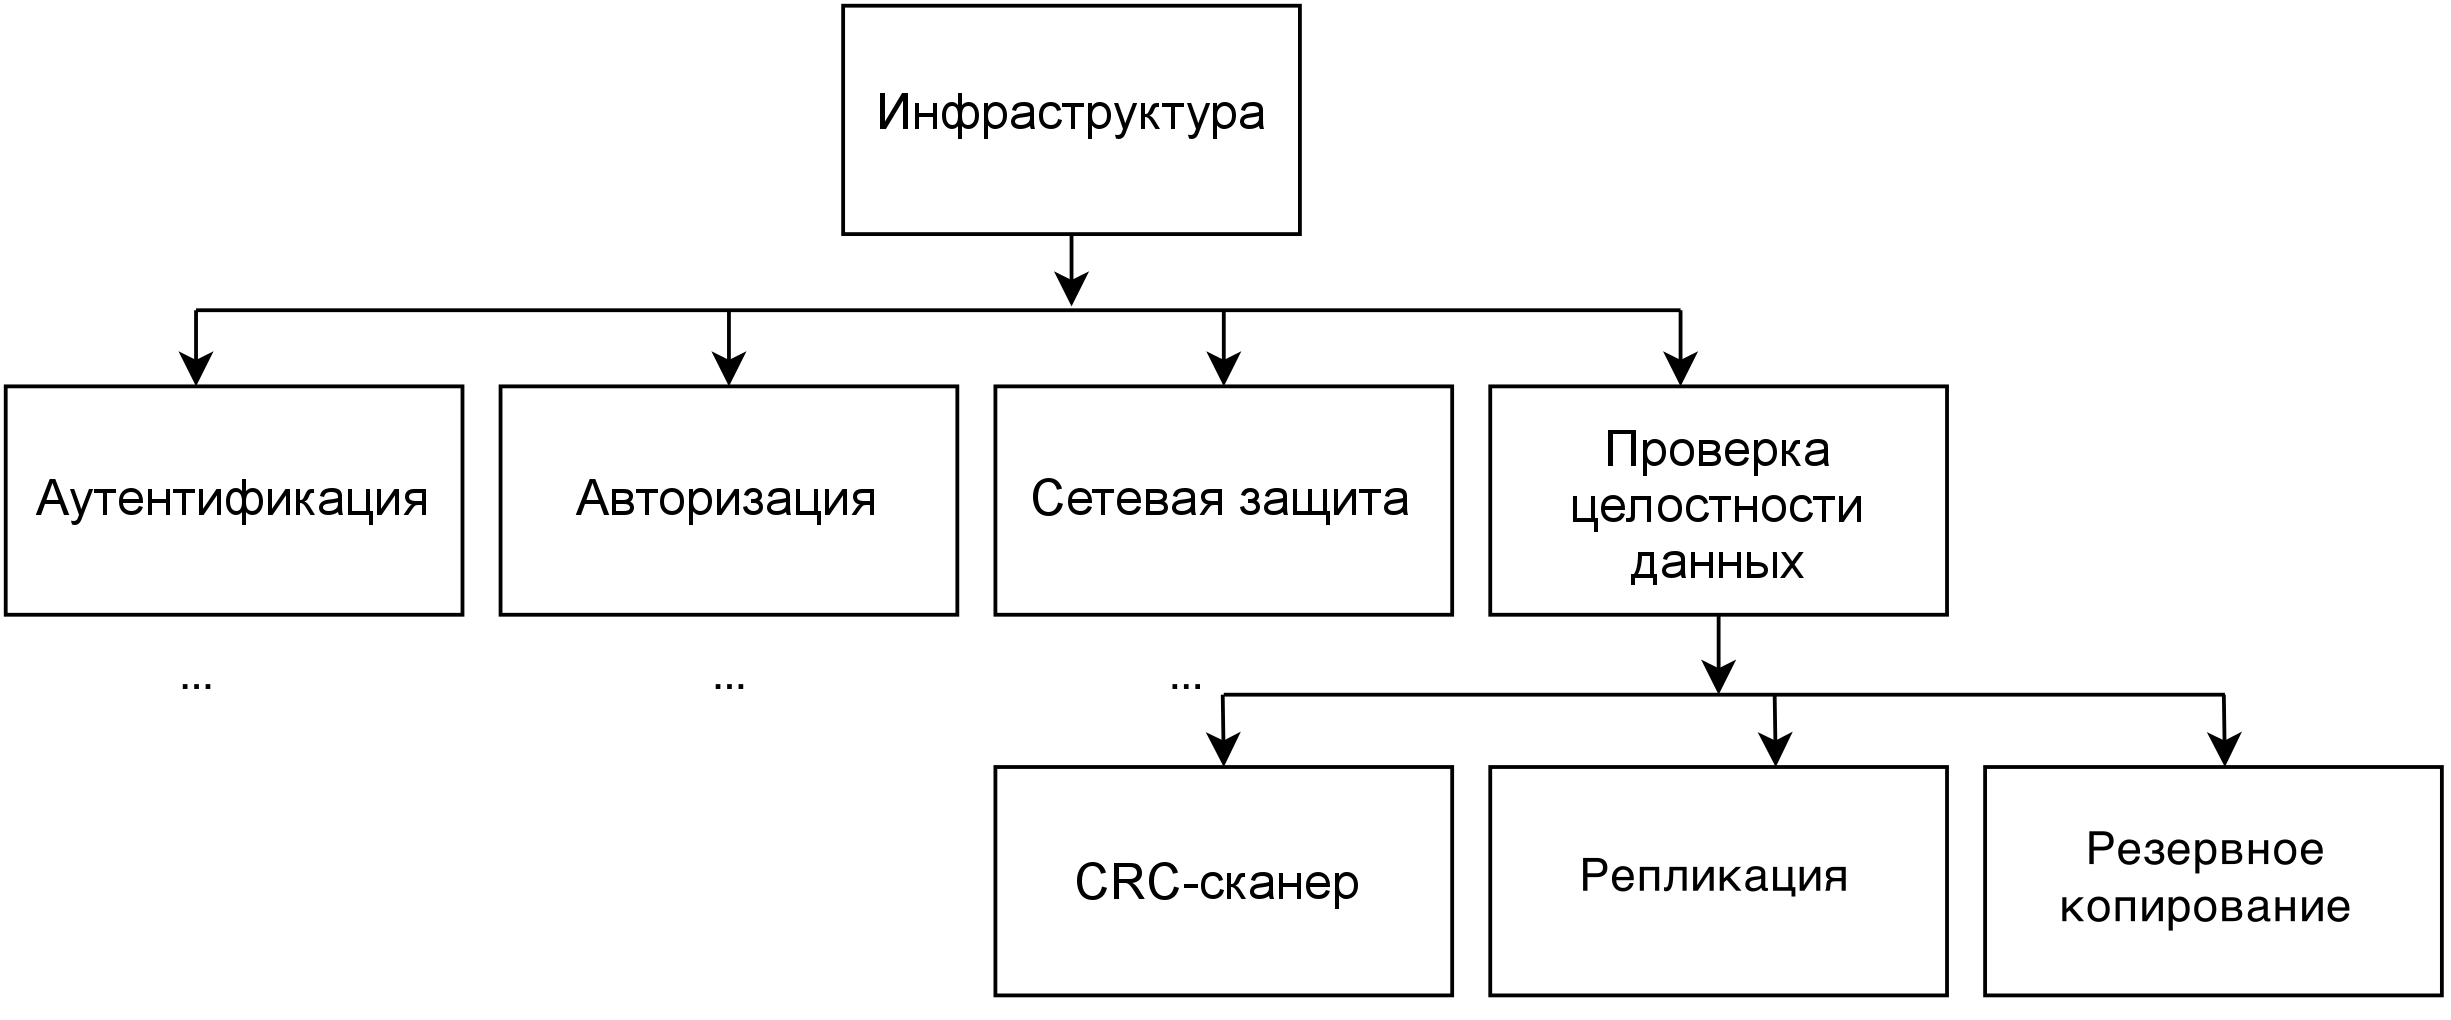
\includegraphics[width=\linewidth]{hierarchy}
\end{figure}
\end{frame}

%-------------------------------------------------------------------------------

\section{Результаты вариантного анализа}

\begin{frame}
\frametitle{\insertsection}

\textbf{Цель:} выбор гипервизора

Метод анализа иерархий:
\begin{itemize}
    \item альтернативы: KVM, Hyper-V, VMware vSphere
    \item критерии: цена, масштабируемость, отказоустойчивость, интерфейсы управления
    \item предпочтение отдано альтернативе В (VMware vSphere)
\end{itemize}

\begin{figure}
    \center
    
\includegraphics[width=\linewidth]{logos-hypervisor}
\end{figure}
\end{frame}

%-------------------------------------------------------------------------------

\section{Структурная схема облачной среды}

\begin{frame}
\frametitle{\insertsection}

\begin{figure}
    \center
    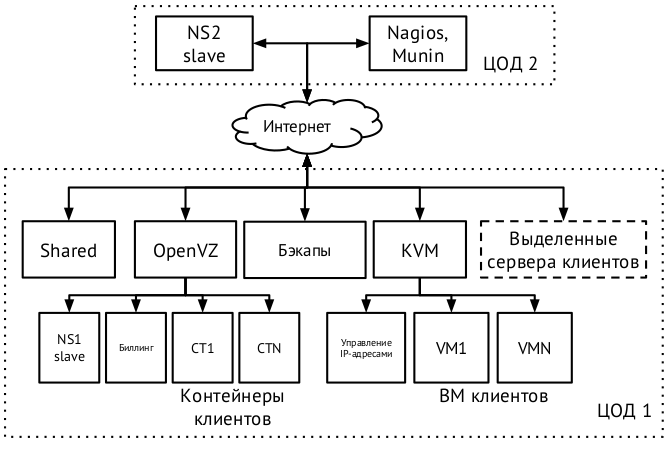
\includegraphics[width=\linewidth]{infrast-scheme}
\end{figure}
\end{frame}

%-------------------------------------------------------------------------------

\section{Архитектура информационной безопасности}

\begin{frame}
\frametitle{\insertsection}

\begin{figure}
    \center
    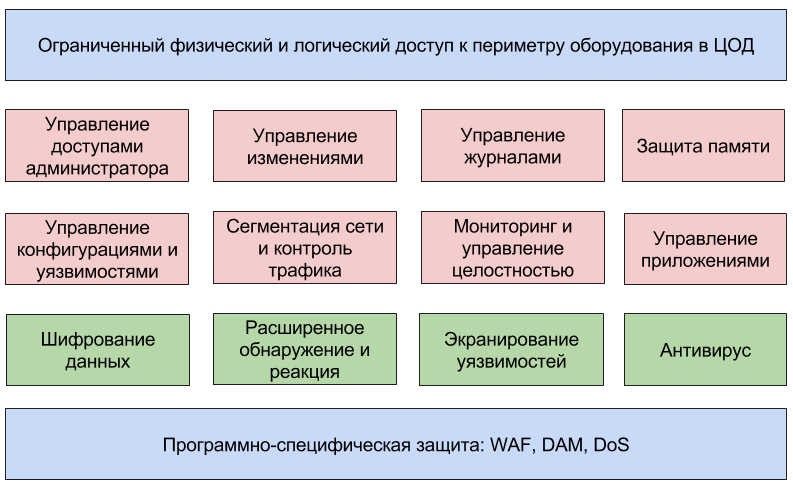
\includegraphics[width=\linewidth]{cwpp}
\end{figure}
\end{frame}

%-------------------------------------------------------------------------------

\section{Экспериментальные исследования}

\begin{frame}
\frametitle{\insertsection}
\framesubtitle{Наиболее опасные критические уязвимости 2016~г.}

\begin{table}[H]
  \begin{tabular}{|l|p{0.8cm}|p{4cm}|l|}
  \hline \textbf{CVE ID} & \textbf{CVSS} & \textbf{Тип уязвимости} & \textbf{ПО} \\
  \hline CVE-2016-5195 & 7.2 & Получение привилегий & Linux Kernel \\
  \hline CVE-2016-6258 & 7.2 & Получение привилегий & Xen \\
  \hline CVE-2016-5696 & 5.8 & Получение данных & Linux Kernel \\
  \hline CVE-2016-3710 & 7.2 & Запуск кода & QEMU \\
  \hline CVE-2016-8655 & 7.2 & Получение привилегий, DoS & Linux Kernel \\
  \hline CVE-2016-4997 & 7.2 & Получение привилегий, доступ к памяти, DoS & Linux Kernel \\
  \hline CVE-2016-4484 & 7.2 & Получение привилегий & CryptSetup \\
  \hline CVE-2016-6309 & 10.0 & DoS, запуск кода & OpenSSL\\
  \hline
  \end{tabular}
\end{table}
\end{frame}

%-------------------------------------------------------------------------------

\section{Экспериментальные исследования}

\begin{frame}
\frametitle{\insertsection}
\framesubtitle{Уведомление скрипта мониторинга в Telegram}

\begin{figure}
    \center
    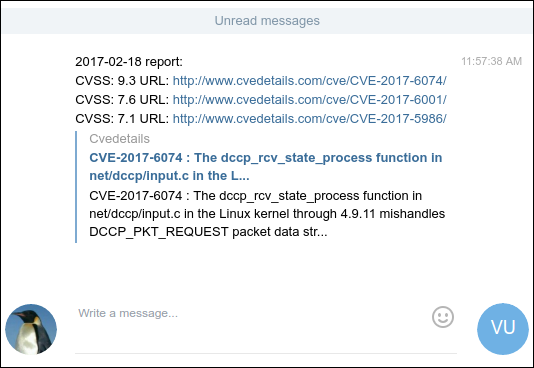
\includegraphics[width=0.9\linewidth]{tscreen}
\end{figure}
\end{frame}

%-------------------------------------------------------------------------------

\section{Результаты}

\begin{frame}
\frametitle{\insertsection}

\begin{itemize}
    \item обзор литературных источников и открытых стандартов
    \item анализ рынка облачных услуг
    \item определение угроз безопасности облачных вычислений и методов их решения
    \item системный анализ безопасности облачной среды
    \item вариантный анализ для выбора оптимальной альтернативы
    \item сбор данных по наиболее опасным уязвимостям в ПО
    \item практическая эксплуатация уязвимости CVE-2016-5195
    \item разработка системы сбора данных по уязвимостям
\end{itemize}
\end{frame}

%-------------------------------------------------------------------------------

\section{Выводы}

\begin{frame}
\frametitle{\insertsection}

\begin{itemize}
    \item проанализированы существующие проблемы и стандарты безопасности облачных вычислений
    \item предложены способы решения данных проблем
    \item рассмотрена специфика предоставления облачных услуг зарубежных и отечественных поставщиков
    \item проанализированы опасные уязвимости за 2016~г.
    \item описаны входные и выходные данные, функции системы безопасности, произведена декомпозиция системы и описана связь между ее элементами
    \item произведен сравнительный анализ гипервизоров
    \item эксплуатирована уязвимость CVE-2016-5195
    \item разработана система мониторинга уязвимостей
\end{itemize}
\end{frame}

%-------------------------------------------------------------------------------
